% !TeX spellcheck = en_GB
% !TeX root = ../../build/zkEVM-architecture.tex

\section{Main State Machine}



\begin{frame}{Main State Machine of a Simplified Virtual Machine}
\begin{figure}
	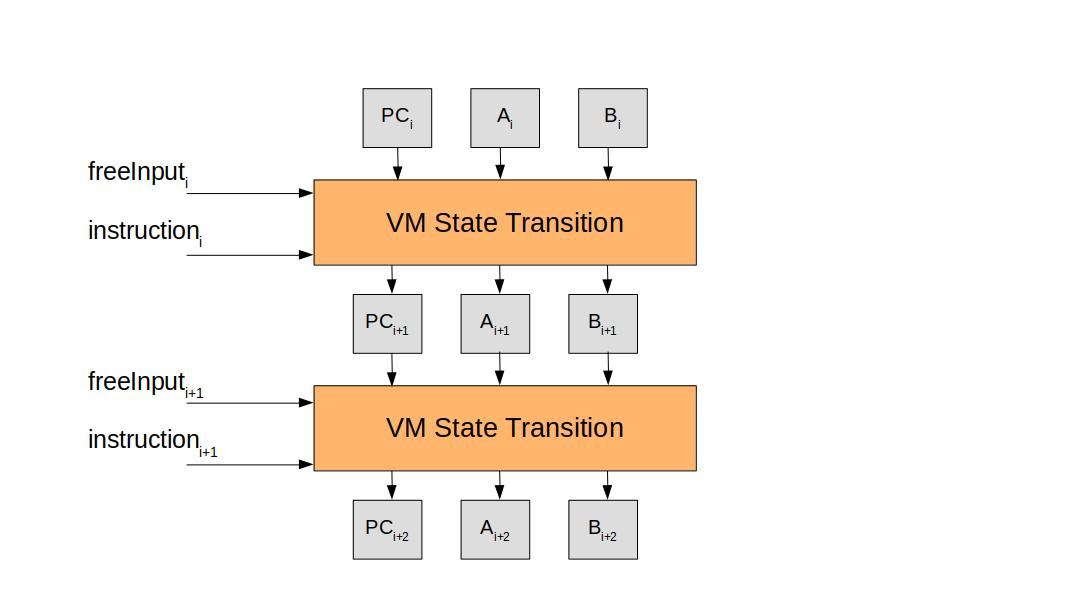
\includegraphics[width=0.65\textwidth]{main-state-machine-simplified-overview}
\end{figure}
\end{frame}
















\begin{frame}[allowframebreaks]{Example Program}
\begin{itemize}
\item Let's now work with a real program:
\[
\begin{array}{|c|l|c|}
\hline
\mathbf{Position} & \multicolumn{2}{|c|}{\mathbf{Instruction}} \\ \hline
0 & \mathbf{FREELOAD} & A \\ \hline
1 & \mathbf{MOV} & B, 3 \\ \hline
2 & \mathbf{JMP}~(if~B = 0) & 6 \\ \hline
3 & \mathbf{MUL} & A, A \\ \hline
4 & \mathbf{DEC} & B \\ \hline
5 & \mathbf{JMP} & 2 \\ \hline
6 & \mathbf{STOP} & \emptyset \\ \hline
\end{array}
\]

\item First, we encode each instruction in hexadecimal as follows:
\begin{columns}
\begin{column}{0.5\textwidth}
\begin{align*}
\mathbf{FREELOAD}~A &\to 0x00010000 \\
\mathbf{MOV}~B,n &\to 0x00020000 + n \\
\mathbf{JMP}~(if~B = 0)~n &\to 0x00040000 + n \\
\mathbf{JMP}~n &\to 0x00080000 + n \\
\mathbf{MUL}~A,A &\to 0x00100000 \\
\mathbf{DEC}~B &\to 0x00200000 \\
\mathbf{STOP} &\to 0x00400000 
\end{align*}
\end{column}
\begin{column}{0.5\textwidth}
\[
\begin{array}{|c|l|c|c|}
\hline
\mathbf{Position} & \multicolumn{2}{|c|}{\mathbf{Instruction}} & \mathbf{Inst.~Value}\\ \hline
0 & \mathbf{FREELOAD} & A & 0x00010000 \\ \hline
1 & \mathbf{MOV} & B, 3 & 0x00020003 \\ \hline
2 & \mathbf{JMP}~(if~B = 0) & 6 & 0x00040006 \\ \hline
3 & \mathbf{MUL} & A, A & 0x00100000 \\ \hline
4 & \mathbf{DEC} & B & 0x00200000 \\ \hline
5 & \mathbf{JMP} & 2 & 0x00080002 \\ \hline
6 & \mathbf{STOP} & \emptyset & 0x00400000 \\ \hline
\end{array}
\]
\end{column}
\end{columns}

\framebreak
\item With the support of this encoding, now we can compute the whole trace of the execution of this program:
\end{itemize}
\scriptsize
\[
\begin{array}{|c|l|c|c|c|c|c|c|}
\hline
\mathbf{Position} & \multicolumn{2}{|c|}{\mathbf{Instruction}} & \mathbf{Inst.~Value} & \mathbf{freeLoad} & \mathbf{PC} & \mathbf{A} & \mathbf{B} \\ \hline
0 & \mathbf{FREELOAD} & A & 0x00010000 & 10 & 0 & 0 & 0 \\ \hline
1 & \mathbf{MOV} & B, 3 & 0x00020003 & 0 & 1 & 10 & 0 \\ \hline
2 & \mathbf{JMP}~(if~B = 0) & 6 & 0x00040006 & 0 & 2 & 10 & 3 \\ \hline
3 & \mathbf{MUL} & A, A & 0x00100000 & 0 & 3 & 10 & 3 \\ \hline
4 & \mathbf{DEC} & B & 0x00200000 & 0 & 4 & 100 & 3 \\ \hline
5 & \mathbf{JMP} & 2 & 0x00080002 & 0 & 5 & 100 & 2 \\ \hline
6 & \mathbf{JMP}~(if~B = 0) & 6 & 0x00040006 & 0 & 2 & 100 & 2 \\ \hline
7 & \mathbf{MUL} & A, A & 0x00100000 & 0 & 3 & 100 & 2 \\ \hline
8 & \mathbf{DEC} & B & 0x00200000 & 0 & 4 & 1000 & 2 \\ \hline
9 & \mathbf{JMP} & 2 & 0x00080002 & 0 & 5 & 1000 & 1 \\ \hline
10 & \mathbf{JMP}~(if~B = 0) & 6 & 0x00040006 & 0 & 2 & 1000 & 1 \\ \hline
11 & \mathbf{MUL} & A, A & 0x00100000 & 0 & 3 & 1000 & 1 \\ \hline
12 & \mathbf{DEC} & B & 0x00200000 & 0 & 4 & 10000 & 1 \\ \hline
13 & \mathbf{JMP} & 2 & 0x00080002 & 0 & 5 & 10000 & 0 \\ \hline
14 & \mathbf{JMP}~(if~B = 0) & 6 & 0x00040006 & 0 & 2 & 10000 & 0 \\ \hline
15 & \mathbf{STOP} & \emptyset & 0x00400000 & 0 & 6 & 10000 & 0 \\ \hline
\end{array}
\]
\end{frame}





\begin{frame}[allowframebreaks]{Checking the Correct Program Execution}
\begin{itemize}
\item The question that arises now is:
\begin{center}
\textbf{How do we actually verify that we are executing the correct program?}
\end{center}

\item The solution seems obvious: Check that every row of the trace of the execution coincides with some row of the program.

\item Then, the question becomes to:
\begin{center}
\textbf{How do we actually verify that we are executing the correct program \\ in an efficient manner?}
\end{center}

\item We can do it with Plookup!

\framebreak

\item On the one side:
\[
\begin{array}{|c|l|c|c|c|}
\hline
\mathbf{Position} & \multicolumn{2}{|c|}{\mathbf{Instruction}} & \mathbf{Inst.~Value} & \mathbf{Rom} = \mathbf{inst} + 2^{32} \cdot \mathbf{position} \\ \hline
0 & \mathbf{FREELOAD} & A & 0x00010000 & 0x0.00010000 \\ \hline
1 & \mathbf{MOV} & B, 3 & 0x00020003 & 0x1.00020003 \\ \hline
2 & \mathbf{JMP}~(if~B = 0) & 6 & 0x00040006 & 0x2.00040006 \\ \hline
3 & \mathbf{MUL} & A, A & 0x00100000 & 0x3.00100000 \\ \hline
4 & \mathbf{DEC} & B & 0x00200000 & 0x4.00200000 \\ \hline
5 & \mathbf{JMP} & 2 & 0x00080002 & 0x5.00080002 \\ \hline
6 & \mathbf{STOP} & \emptyset & 0x00400000 & 0x6.00400000 \\ \hline
\end{array}
\]

\item On the other side:
\scriptsize
\[
\begin{array}{|c|l|c|c|c|c|c|c|c|}
\hline
\mathbf{Position} & \multicolumn{2}{|c|}{\mathbf{Instruction}} & \mathbf{Inst.~Value} & \mathbf{freeLoad} & \mathbf{PC} & \mathbf{A} & \mathbf{B} &  \mathbf{instTrace} = \mathbf{inst} + 2^{32} \cdot \mathbf{PC} \\ \hline
0 & \mathbf{FREELOAD} & A & 0x00010000 & 10 & 0 & 0 & 0 & 0x0.00010000 \\ \hline
1 & \mathbf{MOV} & B, 3 & 0x00020003 & 0 & 1 & 10 & 0 & 0x1.00020003 \\ \hline
2 & \mathbf{JMP}~(if~B = 0) & 6 & 0x00040006 & 0 & 2 & 10 & 3 & 0x2.00040006 \\ \hline
3 & \mathbf{MUL} & A, A & 0x00100000 & 0 & 3 & 10 & 3 & 0x3.00100000 \\ \hline
4 & \mathbf{DEC} & B & 0x00200000 & 0 & 4 & 100 & 3 & 0x4.00200000 \\ \hline
5 & \mathbf{JMP} & 2 & 0x00080002 & 0 & 5 & 100 & 2 & 0x5.00080002 \\ \hline
6 & \mathbf{JMP}~(if~B = 0) & 6 & 0x00040006 & 0 & 2 & 100 & 2 & 0x2.00040006 \\ \hline
7 & \mathbf{MUL} & A, A & 0x00100000 & 0 & 3 & 100 & 2 & 0x3.00100000 \\ \hline
8 & \mathbf{DEC} & B & 0x00200000 & 0 & 4 & 1000 & 2 & 0x4.00200000 \\ \hline
9 & \mathbf{JMP} & 2 & 0x00080002 & 0 & 5 & 1000 & 1 & 0x5.00080002 \\ \hline
10 & \mathbf{JMP}~(if~B = 0) & 6 & 0x00040006 & 0 & 2 & 1000 & 1 & 0x2.00040006 \\ \hline
11 & \mathbf{MUL} & A, A & 0x00100000 & 0 & 3 & 1000 & 1 & 0x3.00100000 \\ \hline
12 & \mathbf{DEC} & B & 0x00200000 & 0 & 4 & 10000 & 1 & 0x4.00200000 \\ \hline
13 & \mathbf{JMP} & 2 & 0x00080002 & 0 & 5 & 10000 & 0 & 0x5.00080002 \\ \hline
14 & \mathbf{JMP}~(if~B = 0) & 6 & 0x00040006 & 0 & 2 & 10000 & 0 & 0x2.00040006 \\ \hline
15 & \mathbf{STOP} & \emptyset & 0x00400000 & 0 & 6 & 10000 & 0 & 0x6.00400000 \\ \hline
\end{array}
\]

\normalsize
\item So, to check that the correct program is being executed, we simply have to use Plookup to determine if:
\[
\mathbf{instTrace} \subset \mathbf{Rom}
\]

\item In simple words, the trace being executed is an execution of the actual program if the instruction trace is contained in the ROM of the program.
\end{itemize}
\end{frame}









\subsection{Storage}
\begin{frame}{Main State Machine of a Virtual Machine}
\begin{figure}
	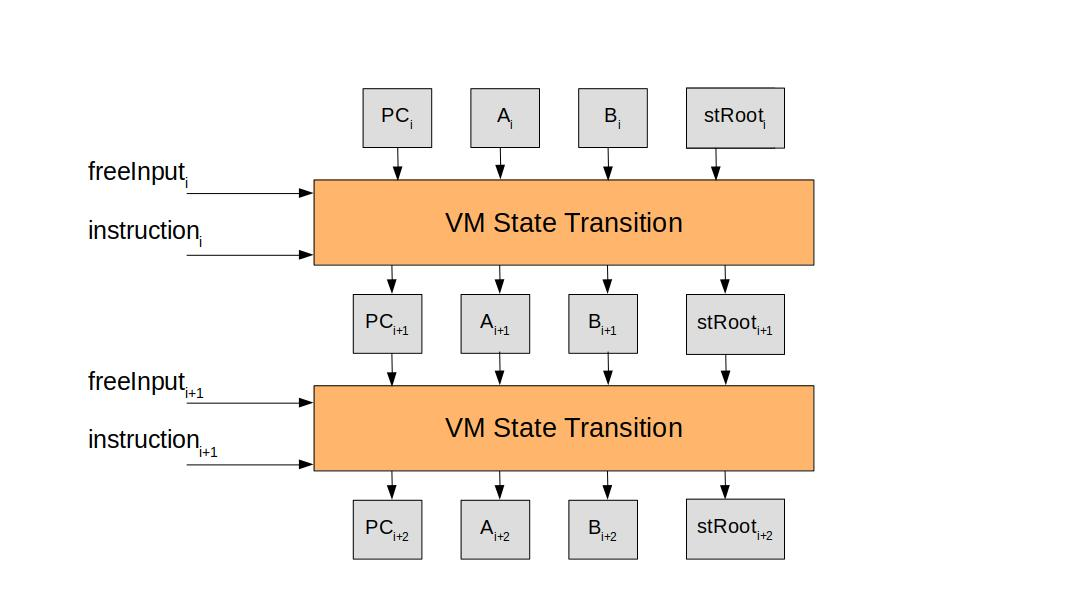
\includegraphics[width=0.65\textwidth]{main-state-machine-overview}
\end{figure}
\end{frame}







\begin{frame}{Main State Machine of a Virtual Machine}
\scriptsize
\[
\begin{array}{|c|l|c|c|c|c|c|c|c|c|c|c|}
\hline
\mathbf{Position} & \multicolumn{2}{|c|}{\mathbf{Instruction}} & \mathbf{freeLoad} & \mathbf{stRoot} & \mathbf{A} & \mathbf{B} & \mathbf{oldStRoot} & \mathbf{newStRoot} & \mathbf{Key} & \mathbf{Value} \\ \hline
0 &  &  &  & \mathsf{st1} &  &  & 0 & 0 & 0 & 0 \\ \hline
1 &  &  &  & \mathsf{st1} &  &  & 0 & 0 & 0 & 0 \\ \hline
2 &  &  &  & \mathsf{st1} &  &  & 0 & 0 & 0 & 0 \\ \hline
3 & \mathbf{SSTORE} & [A], B & \mathsf{st2} & \mathsf{st1} & 0x4C76 & 1232 & \mathsf{st1} & \mathsf{st2} & 0x4C76 & 1232 \\ \hline
4 &  &  &  & \mathsf{st2} & 0x4C76 & 1232 & 0 & 0 & 0 & 0 \\ \hline
5 &  &  &  & \mathsf{st2} &  &  & 0 & 0 & 0 & 0 \\ \hline
6 &  &  &  & \mathsf{st2} &  &  & 0 & 0 & 0 & 0 \\ \hline
7 & \mathbf{SSTORE} & [A], B & \mathsf{st3} & \mathsf{st2} & 0x8E12 & 7765 & \mathsf{st2} & \mathsf{st3} & 0x8E12 & 7765 \\ \hline
8 &  &  &  & \mathsf{st3} & 0x8E12 & 7765 & 0 & 0 & 0 & 0 \\ \hline
9 &  &  &  & \mathsf{st3} &  &  & 0 & 0 & 0 & 0 \\ \hline
10 & \mathbf{SSTORE} & [A], B & \mathsf{st4} & \mathsf{st3} & 0xAA23 & 9812 & \mathsf{st3} & \mathsf{st4} & 0xAA23 & 9812 \\ \hline
11 &  &  &  & \mathsf{st4} & 0xAA23 & 9812 & 0 & 0 & 0 & 0 \\ \hline
12 &  &  &  & \mathsf{st4} &  &  & 0 & 0 & 0 & 0 \\ \hline
13 &  &  &  & \mathsf{st4} &  &  & 0 & 0 & 0 & 0 \\ \hline
14 & \mathbf{SSTORE} & [A], B & \mathsf{st5} & \mathsf{st4} & 0x2213 & 8610 & \mathsf{st4} & \mathsf{st5} & 0x2213 & 8610 \\ \hline
15 &  &  &  & \mathsf{st5} & 0x2213 & 8610 & 0 & 0 & 0 & 0 \\ \hline
\end{array}
\]
\end{frame}







\subsection{Memory}


\begin{frame}{Memory in the Main State Machine}
\scriptsize
\[
\begin{array}{|c|l|c|c|c|c|c|c|c|c|c|}
\hline
\mathbf{Position} & \multicolumn{2}{|c|}{\mathbf{Instruction}} & \mathbf{freeLoad}  & \mathbf{A} & \mathbf{B} & \mathbf{mRead} & \mathbf{mWrite} & \mathbf{Address} & \mathbf{Value} \\ \hline
0 &  &  &  &  &  & 0 & 0 & 0 & 0 \\ \hline
1 &  &  &  &  &  & 0 & 0 & 0 & 0 \\ \hline
2 &  &  &  &  &  & 0 & 0 & 0 & 0 \\ \hline
3 & \mathbf{MWRITE} & [A], B &  & 0x4C76 & 1232 & 0 & 1 & 0x4C76 & 1232 \\ \hline
4 &  &  &  & 0x4C76 & 1232 & 0 & 0 & 0 & 0 \\ \hline
5 & \mathbf{MREAD} & B, [A] & 1232 & 0x4C76 & 1232 & 1 & 0 & 0x4C76 & 1232 \\ \hline
6 &  &  &  & 0x4C76 & 1232 & 0 & 0 & 0 & 0 \\ \hline
7 & \mathbf{MWRITE} & [A], B &  & 0x8E12 & 7765 & 0 & 1 & 0x8E12 & 7765 \\ \hline
8 &  &  &  & 0x8E12 & 7765 & 0 & 0 & 0 & 0 \\ \hline
9 &  &  &  &  &  & 0 & 0 & 0 & 0 \\ \hline
10 & \mathbf{MWRITE} & [A], B &  & 0x2213 & 8610 & 0 & 1 & 0x2213 & 8610 \\ \hline
11 &  &  &  & 0x2213 & 8610 & 0 & 0 & 0 & 0 \\ \hline
12 &  &  &  &  &  & 0 & 0 & 0 & 0 \\ \hline
13 &  &  &  &  &  & 0 & 0 & 0 & 0 \\ \hline
14 & \mathbf{MREAD} & B, [A] & 7765 & 0x8E12 & 7765 & 1 & 0 & 0x8E12 & 7765 \\ \hline
15 &  &  &  & 0x8E12 & 7765 & 0 & 0 & 0 & 0 \\ \hline
\end{array}
\]
\end{frame}







\begin{frame}{Memory State Machine}
\scriptsize
\[
\begin{array}{|c|l|c|c|c|c|c|c|c|}
\hline
\multicolumn{5}{|c|}{\textbf{Free Inputs}} & \multicolumn{2}{|c|}{\textbf{Intermediary State}} & \mathbf{Results} \\ \hline
\mathbf{Position} & \textbf{mRead} & \textbf{mWrite} & \mathbf{Address}  & \mathbf{ValueIn} & \mathbf{stOld} & \mathbf{stNew} & \mathbf{Value} \\ \hline
%0 & 0 & 0 & 0 & 0 & 0 & 0 & 0 \\ \hline
3 & 0 & 1 & 0x4C76 & 1232 & 0 & 1232 & 1232 \\ \hline
5 & 1 & 0 & 0x4C76 &  & 1232 & 1232 & 1232 \\ \hline
7 & 0 & 1 & 0x8E12 & 7765 & 1232 & 7765 & 7765 \\ \hline
14 & 1 & 0 & 0x8E12 &  & 7765 & 7765 & 7765 \\ \hline
10 & 0 & 1 & 0x2213 & 8610 & 7765 & 8610 & 8610 \\ \hline
\end{array}
\]
\small
\begin{itemize}
\item Using Plookup, prove that the polynomial:
\[
main.position(x) + v \cdot main.mRead(x) + v^2 \cdot main.mWrite(x) + v^3 \cdot main.Address(x) + v^4 \cdot main.Value(x),
\]
is included in the polynomial:
\[
mem.position(x) + v \cdot mem.mRead(x) + v^2 \cdot mem.mWrite(x) + v^3 \cdot mem.Address(x) + v^4 \cdot mem.Value(x).
\]
\end{itemize}
\end{frame}







\subsection{Binary Operations}

\begin{frame}{Checking Binary Operations: XOR}
\begin{columns}
\footnotesize
\begin{column}{0.5\textwidth}
\begin{center}
\underline{\textbf{Operation}} \\[0.2cm]
$f(x) \xor g(x) = h(x)$.
\end{center}
\begin{enumerate}
\item Check byte decomposition:
\begin{align*}
f(x) &= f_0(x) + 2^8 f_1(x) + 2^{16} f_2(x) + \dots \\
g(x) &= g_0(x) + 2^8 g_1(x) + 2^{16} g_2(x) + \dots \\
h(x) &= h_0(x) + 2^8 h_1(x) + 2^{16} h_2(x) + \dots
\end{align*}

\item Check byte form elementwise:
\[
\begin{array}{ccc}
f_0(x) \subset \mathsf{byte(x)} & g_0(x) \subset \mathsf{byte(x)} & h_0(x) \subset \mathsf{byte(x)} \\
f_1(x) \subset \mathsf{byte(x)} & g_1(x) \subset \mathsf{byte(x)} & h_1(x) \subset \mathsf{byte(x)} \\
f_2(x) \subset \mathsf{byte(x)} & g_2(x) \subset \mathsf{byte(x)} & h_2(x) \subset \mathsf{byte(x)} \\
\vdots & \vdots & \vdots
\end{array}
\]
\end{enumerate}
\end{column}
\begin{column}{0.5\textwidth}
\begin{enumerate}
\item[3.] Check $\XOR$ operation:
\[
\begin{array}{c}
f_0(x) + 2^8 g_0(x) + 2^{16} h_0(x) \subset \XOR(x) \\
f_1(x) + 2^8 g_1(x) + 2^{16} h_1(x) \subset \XOR(x) \\
f_2(x) + 2^8 g_2(x) + 2^{16} h_2(x) \subset \XOR(x) \\
\vdots
\end{array}
\]
\end{enumerate}
\[
\begin{array}{|c|c|}
\hline
\mathbf{x} & \mathbf{byte} \\ \hline
\omega^0 & 0x00 \\ \hline
\omega^1 & 0x01 \\ \hline
\vdots & \vdots \\ \hline
\omega^{123} & 0x7B \\ \hline
\vdots & \vdots \\ \hline
\omega^{255} & 0xFF \\ \hline
\end{array}
\hspace{1cm}
\begin{array}{|c|c|}
\hline
\mathbf{x} & \XOR \\ \hline
\omega^0 & 0x000000 \\ \hline
\omega^1 & 0x010001 \\ \hline
\vdots & \vdots \\ \hline
\omega^{5028} & 0xB713A4 \\ \hline
\vdots & \vdots \\ \hline
\omega^{65535} & 0x00FFFF \\ \hline
\end{array}
\]
\end{column}
\end{columns}
\end{frame}










\subsection{Arithmetic Operations}

\begin{frame}{Checking Arithmetic Operations: Multiplication}
\scriptsize
\begin{columns}
\begin{column}{0.5\textwidth}
\begin{figure}
	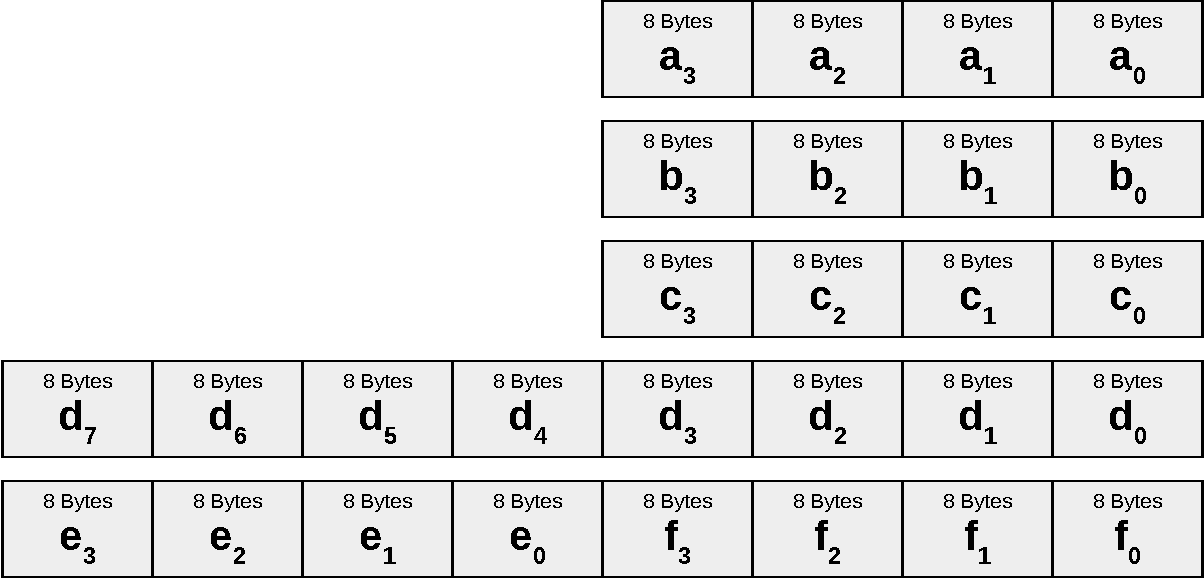
\includegraphics[width=0.8\textwidth]{multiplication}
\end{figure}
\end{column}
\begin{column}{0.5\textwidth}
\begin{align*}
A = &~a_2 \cdot 256^{22} + a_1 \cdot 256^{11} + a_0, \\
B = &~b_2 \cdot 256^{22} + b_1 \cdot 256^{11} + b_0, \\
C = &~c_2 \cdot 256^{22} + c_1 \cdot 256^{11} + c_0, \\
D = &~d_5 \cdot 256^{55} + d_4 \cdot 256^{44} + d_3 \cdot 256^{33} \\
&+ d_2 \cdot 256^{22} + d_1 \cdot 256^{11} + d_0, \\
E = &~e_2 \cdot 256^{22} + e_1 \cdot 256^{11} + e_0, \\
F = &~f_2 \cdot 256^{22} + f_1 \cdot 256^{11} + f_0,
\end{align*}
\end{column}
\end{columns}
\begin{columns}
\begin{column}{0.33\textwidth}
\[
A \cdot B + C = D = E \cdot 2^{256} + F
\]
\end{column}
\begin{column}{0.33\textwidth}
\begin{align*}
&d_0 = f_0, \\
&d_1 = f_1, \\
&d_2 = f_2 + \mathsf{carry_1} \cdot 256^{10}, \\
&d_3 \cdot 256 + \mathsf{carry_1} = e_0 + \mathsf{carry_2} \cdot 256^{11}, \\
&d_4 \cdot 256 + \mathsf{carry_2} = e_1 + \mathsf{carry_3} \cdot 256^{11}, \\
&d_5 \cdot 256 + \mathsf{carry_3} = e_1.
\end{align*}
\end{column}
\begin{column}{0.33\textwidth}
\[
\mathsf{carry_1}, \mathsf{carry_2}, \mathsf{carry_3} \subset \mathsf{byte}.
\]
\end{column}
\end{columns}
\end{frame}









\begin{frame}{Multiplying}
\scriptsize
\[
\begin{array}{|c|c|c|c|c|c|c|c|c|c|c|c|c|c|c|c|c|c|c|}
\hline
\mathbf{Step} & \mathbf{mA} & \mathbf{mB} & \mathbf{acc_5} & \mathbf{acc_4}  & \mathbf{acc_3} & \mathbf{acc_2} & \mathbf{acc_1} & \mathbf{acc_0} \\ \hline
0 & a_0 & b_0 & d_5 & d_4 & d_3 & d_2 & d_1 & d_0 \\ \hline
1 & a_0 & b_1 & d_0 & d_5 & d_4 & d_3 & d_2 & d_1 \\ \hline
2 & a_1 & b_0 & d_0 & d_5 & d_4 & d_3 & d_2 & d_1 \\ \hline
3 & a_0 & b_2 & d_1 & d_0 & d_5 & d_4 & d_3 & d_2 \\ \hline
4 & a_1 & b_1 & d_1 & d_0 & d_5 & d_4 & d_3 & d_2 \\ \hline
5 & a_2 & b_0 & d_1 & d_0 & d_5 & d_4 & d_3 & d_2 \\ \hline
6 & a_1 & b_2 & d_2 & d_1 & d_0 & d_5 & d_4 & d_3 \\ \hline
7 & a_2 & b_1 & d_2 & d_1 & d_0 & d_5 & d_4 & d_3 \\ \hline
8 & a_2 & b_2 & d_3 & d_2 & d_1 & d_0 & d_5 & d_4 \\ \hline
\end{array}
\]
\[
\hspace{2.5cm}
\begin{array}{|c|c|c|c|c|c|c|c|c|c|c|c|c|c|c|c|c|c|c|}
\hline
\mathbf{q_{shift}} & \mathbf{q_{same}} & \mathbf{q_{set}} & \mathbf{q_{result}} & \mathbf{q_{a_0}} & \mathbf{q_{a_1}} & \mathbf{q_{a_2}} & \mathbf{q_{b_0}} & \mathbf{q_{b_1}} & \mathbf{q_{b_2}} \\ \hline
0 & 0 & 1 & 0 & 1 & 0 & 0 & 1 & 0 & 0\\ \hline
1 & 0 & 0 & 0 & 1 & 0 & 0 & 0 & 1 & 0\\ \hline
0 & 1 & 0 & 0 & 0 & 1 & 0 & 1 & 0 & 0\\ \hline
1 & 0 & 0 & 0 & 1 & 0 & 0 & 0 & 0 & 1\\ \hline
0 & 1 & 0 & 0 & 0 & 1 & 0 & 0 & 1 & 0\\ \hline
0 & 1 & 0 & 0 & 0 & 0 & 1 & 1 & 0 & 0\\ \hline
1 & 0 & 0 & 0 & 0 & 1 & 0 & 0 & 0 & 1\\ \hline
0 & 1 & 0 & 0 & 0 & 0 & 1 & 0 & 1 & 0\\ \hline
1 & 0 & 0 & 1 & 0 & 0 & 1 & 0 & 0 & 1\\ \hline
\end{array}
\]
\end{frame}
